\documentclass[crop,tikz]{standalone}
\usetikzlibrary{backgrounds}
\colorlet{blue}{cyan}
\tikzset{
  inverted/.style = {
    color=white,
    background rectangle/.style={fill},
    show background rectangle
  }
}
\usepackage{pgfplots}
\pgfplotsset{compat=1.13}

\pgfplotsset{
  inverted/.style = {
    every axis legend/.append style={
      draw=white,
      fill=black,
      text=white
    }
  },
  every non boxed x axis/.append style={
    axis line style={-latex}
  },
  every non boxed y axis/.append style={
    axis line style={-latex}
  }
}

\begin{document}
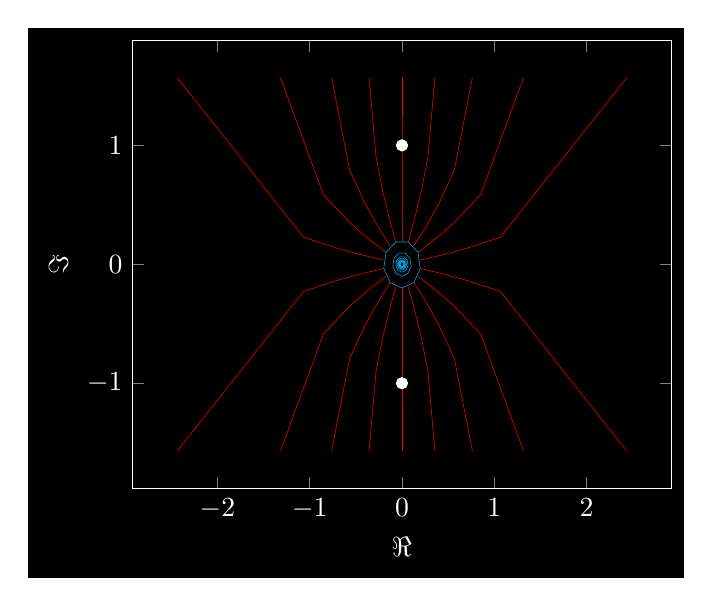
\begin{tikzpicture}[inverted,inverted]
  \pgfmathsetmacro{\numberoffieldlines}{40};
  \pgfmathsetmacro{\numberofpotentiallines}{30};
  \pgfmathsetmacro{\charge}{1};
  \pgfmathsetmacro{\chargedistance}{1};
  \pgfmathsetmacro{\remin}{-4};
  \pgfmathsetmacro{\remax}{4};
  \pgfmathsetmacro{\immin}{-4};
  \pgfmathsetmacro{\immax}{4};
  \begin{axis}[inverted,
    % axis equal image,
    % xmin={\remin}, xmax={\remax},
    % ymin={\immin}, ymax={\immax},
    % ytick={-2*pi,-pi,0,pi,2*pi},
    % yticklabels={$-2\pi$,$-\pi$,$0$,$\pi$,$2\pi$},
    xlabel={$\Re$},
    ylabel={$\Im$},
    samples=10,
    declare function = {
      rephi(\p,\r,\a) = \charge*0.5*ln((\r^2*cos(\p)^2 + (\r*sin(\p) - \a)^2)/(\r^2*cos(\p)^2 + (\r*sin(\p) + \a)^2));
      imphi(\p,\r,\a) = \charge*rad(atan2(-2*\a*\r*cos(\p)/(\a^2 + \r^2 + 2*\a*\r*sin(\p)), (\r^2 - \a^2)/(\a^2 + \r^2 + 2*\a*\r*sin(\p))));
      % imphi(\p,\r,\a) = \charge*rad(atan(-2*\a*\r*cos(\p)/(\r^2 - \a^2)));
    },
    clip=false,
    ]
    % field lines
    \pgfplotsinvokeforeach{0,20,...,360}{
      \addplot[red,very thin,domain=1:10] ({rephi(#1,x,\chargedistance)},{imphi(#1,x,\chargedistance)});
    }
    % lines of constant potential
    \pgfplotsinvokeforeach{10,20,...,100}{
      \addplot[blue,very thin,domain=0:360] ({rephi(x,#1,\chargedistance)},{imphi(x,#1,\chargedistance)});
    }
    % charges
    \addplot[only marks,mark=*] coordinates { (0,{ \chargedistance}) };
    \addplot[only marks,mark=*] coordinates { (0,{-\chargedistance}) };
  \end{axis}
\end{tikzpicture}
\end{document}
